\documentclass[a4paper,14pt]{extarticle}

\usepackage[utf8x]{inputenc}
\usepackage[T1,T2A]{fontenc}
\usepackage[russian]{babel}
\usepackage{hyperref}
\usepackage{indentfirst}
\usepackage{here}
\usepackage{array}
\usepackage{graphicx}
\usepackage{caption}
\usepackage{subcaption}
\usepackage{chngcntr}
\usepackage{amsmath}
\usepackage{amssymb}
\usepackage{pgfplots}
\usepackage{pgfplotstable}
\usepackage[left=2cm,right=2cm,top=2cm,bottom=2cm,bindingoffset=0cm]{geometry}
\usepackage{multicol}
\usepackage{askmaps}
\usepackage{enumitem}

\setitemize{itemsep=0em}
\setenumerate{itemsep=0em}

\renewcommand{\le}{\ensuremath{\leqslant}}
\renewcommand{\leq}{\ensuremath{\leqslant}}
\renewcommand{\ge}{\ensuremath{\geqslant}}
\renewcommand{\geq}{\ensuremath{\geqslant}}
\renewcommand{\epsilon}{\ensuremath{\varepsilon}}
\renewcommand{\phi}{\ensuremath{\varphi}}
\renewcommand{\thefigure}{\arabic{figure}} 	
\renewcommand*\not[1]{\overline{#1}}

%\titleformat*{\section}{\large\bfseries} 
%\titleformat*{\subsection}{\normalsize\bfseries} 
%\titleformat*{\subsubsection}{\normalsize\bfseries} 
%\titleformat*{\paragraph}{\normalsize\bfseries} 
%\titleformat*{\subparagraph}{\normalsize\bfseries} 

\counterwithin{figure}{section}
\counterwithin{equation}{section}
\counterwithin{table}{section}
\newcommand{\sign}[1][5cm]{\makebox[#1]{\hrulefill}}
\graphicspath{{../pics/}}
\captionsetup{justification=centering,margin=1cm}
\def\arraystretch{1.3}
\setlength\parindent{5ex}
%\titlelabel{\thetitle.\quad}

\begin{document}

\begin{titlepage}
\begin{center}
	Санкт-Петербургский Политехнический Университет Петра Великого\\[0.3cm]
	Институт компьютерных наук и технологий \\[0.3cm]
	Кафедра компьютерных систем и программных технологий\\[4cm]
	
	\textbf{ОТЧЕТ}\\ 
	\textbf{по лабораторной работе}\\[0.5cm]
	\textbf{<<Исследование персептронов>>}\\[0.1cm]
	\textbf{Нейроинформатика}\\[4.0cm]
\end{center}

\begin{flushright}
	\begin{minipage}{0.45\textwidth}
		\textbf{Работу выполнил студент}\\[3mm]
		группа 33501/4 \hspace*{10mm} Дьячков В.В.\\[5mm]
		\textbf{Преподаватель}\\[5mm]
		\sign[1.7cm] \hspace*{1mm} к.т.н., доц. Никитин К.В. \\[5mm]
	\end{minipage}
\end{flushright}

\vfill

\begin{center}
	Санкт-Петербург\\
	\the\year
\end{center}
\end{titlepage}

\addtocounter{page}{1}

\tableofcontents
\newpage

\section{Цели работы}

Изучение и приобретение навыков:
\begin{itemize}
	\item инициализации НС;
	\item использования функций обработки входных/выходных сигналов;
	\item задания различных функций расчета производительности НС;
	\item задания различных функций деления выборки;
	\item практического применения сетей прямого распространения (НСПР);
	\item обучения НСПР по алгоритму обратного распространения (ОР).
\end{itemize}

\section{Изучение вспомогательных функций}

\subsection{Изучение функций инициализации}

%1. С помощью команды network создайте НС с n входами, 1 выходным слоем с m нейронами.
%Задайте функцию инициализации НС initlay.
%2. Задайте функцию инициализации слоев initnw. Произведите инициализацию НС с помощью функции init. Проанализируйте матрицы смещений и весов нейронной сети.
%3. Задайте функцию инициализации слоев initwb.
%Задавайте для весов и смещений различные функции инициализации (initzero, rands, randsmall – и для весов и для смещений, midpoint, randnc, randnr, initlvq, initsompc – только для весов, initcon – только для смещений). Произведите инициализацию НС с помощью функции init. Проанализируйте матрицы смещений и весов нейронной сети.

Создадим нейронную сеть с 3 входами и одним выходным слоем, содержащим 2 нейрона. Таким образом имеем 3 коэффициента входного слоя \code{net.IW\{1,1\}}, 2 коэффициента весов между входным и выходным слоями \code{net.LW\{2,1\}} и по 1 коэффициенту смещения на каждом слое \code{net.b\{1\}} и \code{net.b\{1\}}, т.е. всего 7 коэффициентов.

%\lstinputlisting[linerange={7-10}]{lab3_1_1.m}

Зададим функцию инициализации слоев \code{'initnw'}. Эта функция генерирует начальные веса и смещения для слоя так, чтобы активные области нейронов были распределены равномерно относительно области входов, что обеспечивает минимизацию числа нейронов сети и времени обучения.

\lstinputlisting[linerange={19-24}]{lab3_1_1.m}

В результате коэффициенты оказались равны:
\begin{gather*}
IW_{1,1} = \begin{bmatrix} -0.5254 & -0.0823 & 0.9262 \end{bmatrix}^T,\
b_1 = \begin{bmatrix} 0.0936 & 0.0423 & -0.5368 \end{bmatrix}^T \\
LW_{2,1} = \begin{bmatrix} -0.0222 & 0.3583 & -0.2651 \\ 0.2481 & -0.2090 & 0.9760 \end{bmatrix},\ 
b_2 = \begin{bmatrix} -0.9245 \\ 0.7703 \end{bmatrix}
\end{gather*}

Зададим функцию инициализации слоев \code{'initwb'}, которая позволяет использовать собственные функции инициализации для каждой матрицы весов и каждого вектора смещений. 

\lstinputlisting[linerange={26-35}]{lab3_1_1.m}

Зададим различные функции инициализации коэффициентов, например при \code{iw11 = 'rands'}, \code{b1 = 'randsmall'}, \code{lw11 = 'initlvq'} и \code{b2 = 'initzero'} коэффициенты оказались равны:
\begin{gather*}
IW_{1,1} = \begin{bmatrix} -0.4763 & -0.3293 & 0.3595 \end{bmatrix}^T,\
b_1 = \begin{bmatrix} 0.0004 & -0.0081 & 0.0064 \end{bmatrix}^T \\
LW_{2,1} = \begin{bmatrix} 1 & 0 & 0 \\ 0 & 1 & 1 \end{bmatrix},\ 
b_2 = \begin{bmatrix} 0 \\ 0 \end{bmatrix}
\end{gather*}

Таким образом были рассмотрены различные функции инициализации коэффициентов и смещений слоев нейронной сети.

\subsection{Изучение функций предобработки входов/выходов}

%Задавайте в качестве функций предобработки различные встроенные функции (fixunknowns, mapminmax, mapstd, processpca, removeconstantrows, removerows) – по очереди по одной.
%Для каждой из функций предобработки подберите актуальные входные примеры, на которые эти функции должны срабатывать (для fixunknowns например задайте в качестве одного из входных сигналов NaN). Подайте эти примеры на вход этих функций и проанализируйте обработанные функциями примеры.

Рассмотрим работу основных встроенных функций предобработки.
\begin{itemize}
	\item \code{fixunknowns(X)} помечает строки, содержащие \code{NaN} и заменят такие элементы на среднее значение в строке. Например, подать матрицу \code{X = [1 2 3; 4 NaN 6]}, то функция вернет на одну строку больше: \code{[1 2 3; 4 5 6; 1 0 1]}. В дополнительной строке содержится ноль, если соответствующей ей элемент в предыдущей строке был равен \code{NaN}.
	\item \code{mapminmax(X)} приводит все значения к интервалу $[-1, 1]$. Например, если подать матрицу \code{X = [1 2 3; 6 5 4]}, то функция вернет \code{[-1 0 1; 1 0 -1]}.
	\item \code{mapstd(X)} приводит все строки к такому виду, что среднее строки равно 0, а стандартное отклонение равно 1. Например, если подать матрицу \code{X = [1 2 3; 4 5 6]}, то функция вернет \code{[-1 0 1; -1 0 1]}.
	\item \code{processpca(X)} проводит обработку столбцов матрицы с анализом основных компонент. Например, если подать матрицу \code{X = [1 2 3; 4 5 6]}, то функция вернет \code{[-4.0758 -5.3845 -6.6931; 0.6229 0.0869 -0.4492]}.
	\item \code{removeconstantrows(X)} удаляет из матрицы константные. Например, если подать матрицу \code{X = [3 3 3; 1 2 3]}, то функция вернет \code{[1 2 3]}.
	\item \code{removerows(X, idx)} удаляет из матрицы строки с индексами, содержащимися в \code{idx}. Например, если подать матрицу \code{X = [1 2 3; 4 5 6; 7 8 9], [1, 3])}, то функция вернет \code{[4 5 6]}.
\end{itemize}

\subsection{Изучение функций расчета производительности (усреднения ошибки)}

%Сформируйте различные вектора (матрицы) ошибок E (интерпретируйте их как вектора ошибок НС на тестовой выборке). Размерность E = число выходов * число векторов. Последовательно примените к ним функции mae, mse, sae, sse. Проанализируйте каждый из способов усреднения ошибки (можно ли ему доверять и когда – при каком числе выходов НС и при каком объеме тестовой выборки). Рассмотрите случаи, когда ошибки сильно рознятся по входам/примерам.

Сформируем искусственный вектор ошибок E и будем интерпретировать его как вектор ошибок НС на тестовой выборке. Создадим матрицу размером $2 \times 5$, т.е. содержащую по 2 выходных значения нейронной сети для каждого из 5 тестовых примеров.
\begin{equation*}
E = \begin{bmatrix}
	0 & 1 & 2 & 0 & 30 \\
	10 & 0 & 15 & 0 & 2
\end{bmatrix}
\end{equation*}

Для данной матрицы ошибок значения функции ошибок равны:
\begin{multicols}{4}
	\centering
	\code{mae} = 6 \\
	\code{mse} = 123.4 \\
	\code{sae} = 60 \\
	\code{sse} = 1234
\end{multicols}

Значения функций \code{sae} и \code{sse} в 10 раз (размерность матрицы) больше, чем значения соответствующих им функций \code{mae} и \code{mse}, так как значения ошибок в данном случае не усредняются. Можно заметить, что функции \code{mse} и \code{sse} гораздо более чувствительны к выбросам (элемент 30 в данном случае), соответственно им можно доверять при большом объеме выборки, когда данные выбросы будут нивелированы.

\subsection{Изучение функций деления выборки}

%Для объема выборки Q = 100 примените функции деления выборки divideblock, divideind, divideint, dividerand, dividetrain. Ознакомьтесь с входными параметрами каждой из функций и при исследовании функций меняйте эти параметры. Проанализируйте, как формируются обучающая, тестовая и контрольная выборки для каждой из функций.

Сформируем выборку размером 100 (\code{P = 0.01 : 0.01 : 1}) и применим к ней различные функции для ее деления:
\begin{itemize}
	\item \code{[Ptr, Pval, Ptest] = divideblock(P, 0.5, 0.3, 0.2)} делит выборку блоками, т.е. первые 50\% выборки будет принадлежать множеству \code{Ptr}, следующие за этим блоком 30\% выборки будет принадлежать \code{Pval} и т.д.
	\item \code{[Ptr, Pval, Ptest] = divideind(P, 1:50, 51:80, 81:100)} делит выборку путем задания индексов каждой подвыборки, т.е. подмножеству \code{Ptr} будут принадлежать примеры с индексами от 1 до 50 и т.д.
	\item \code{[Ptr, Pval, Ptest] = divideint(P, 0.5, 0.3, 0.2)} делит выборку перемежающимися блоками, т.е. элементы будут последовательно добавляться в одно из подмножеств.
	\item \code{[Ptr, Pval, Ptest] = dividerand(P, 0.5, 0.3, 0.2)} делит выборку на подмножества случайным образом.
	\item \code{[Ptr, Pval, Ptest] = dividetrain(P)} не делит выборку на подмножества, а добавляет все относит все примеры к тренировочному подмножеству.
\end{itemize}

\section{Аппроксимация статических зависимостей}

\subsection{Формирование обучающей и тестовой выборки}

Сформируем обучающую и тестовую выборки на основе ранее созданных функций. На рис. \ref{fig:2_2} изображены сформированные выборки. Исходная выборка из $100$ примеров была разделена на обучающую и тестовую в соотношении $0.7 : 0.3$.
\vspace{-0.5cm}
\begin{figure}[H]
\begin{center}
	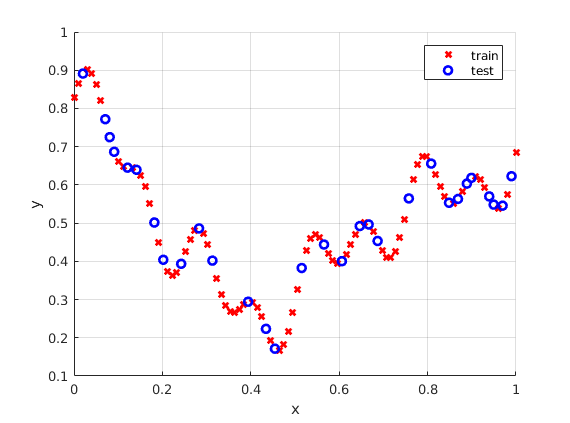
\includegraphics[scale=0.9]{2_2}
	\caption{Обучающая и тестовая выборки}
	\label{fig:2_2}
\end{center}
\end{figure}
\vspace{-1.5cm}

\subsection{Инициализация и критерии останова обучения}

Создадим нейронную сеть с одним скрытым слоем, содержащим 20 нейронов, и инициализируем ее с помощью случайных значений. Зададим ей основные параметры обучения.

\lstinputlisting[linerange={28-37}]{lab3_2_1.m}

\subsection{Обучение НС}

Обучим нейронную сеть на обучающей выборке. На рис. \ref{fig:2_4} изображена зависимость ошибки от номера эпохи.
\begin{figure}[H]
\begin{center}
	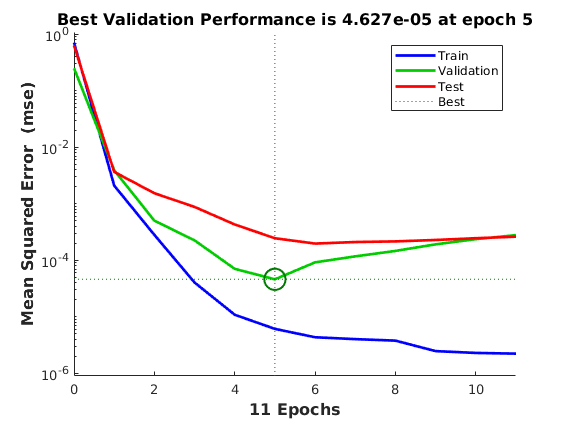
\includegraphics[scale=0.9]{2_4}
	\caption{Зависимость ошибки от номера эпохи}
	\label{fig:2_4}
\end{center}
\end{figure}

Будем изменять количество нейронов в скрытом слое в диапазоне $1 \div 50$ и проверять ошибку на тестовой выборке. 

%\lstinputlisting[linerange={16-26}]{lab3_2_1.m}

На рис. \ref{fig:2_5_1} изображена зависимость ошибки от числа нейронов в скрытом слое.
\begin{figure}[H]
\begin{center}
	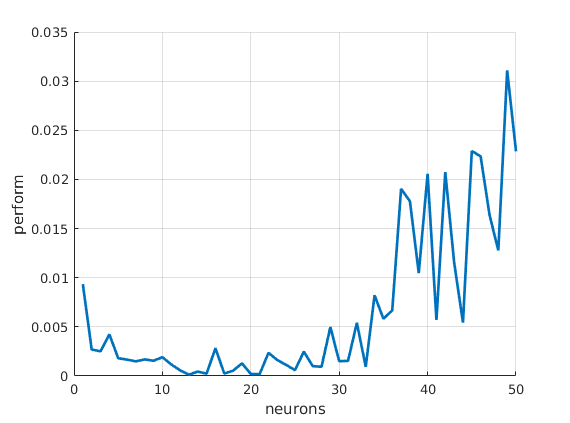
\includegraphics[scale=0.88]{2_5_1}
	\caption{Зависимость ошибки от числа нейронов в скрытом слое}
	\label{fig:2_5_1}
\end{center}
\end{figure}
\vspace{-0.5cm}

Из графика видно, что оптимальное количество нейронов в скрытом слое лежит в диапазоне $10 \div 20$. На рис. \ref{fig:2_5_2} изображены аппроксимации при различном количестве нейронов.
\vspace{-0.5cm}
\begin{figure}[H]
\begin{center}
	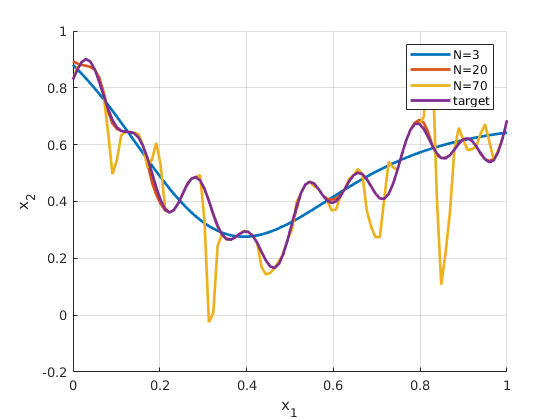
\includegraphics[scale=0.88]{2_5_2}
	\caption{Аппроксимации при различном количестве нейронов}
	\label{fig:2_5_2}
\end{center}
\end{figure}

\subsection{Пакетные алгоритмы обучения}

Применим различные пакетные алгоритмы обучения и подберем для каждого из них оптимальные параметры. В таблице \ref{tab:2_6_1} и на рис. \ref{fig:2_6_1} приведены сводные результаты для градиентных алгоритмов.
\vspace{-0.5cm}
\begin{table}[H]
\begin{center}
	\def\tabcolsep{10pt}
	\caption{Градиентные алгоритмы}
	\label{tab:2_6_1}
	\begin{tabular}{|c|c|c|c|c|}
		\hline
		Функция & Параметры & Нейроны & Ошибка & Число эпох \\
		\hline
		\hline
		\code{traingda} & \makecell{
			\code{lr = 0.01} \\ 
			\code{lr_inc = 1.05} \\ 
			\code{lr_dec = 0.7} \\
			\code{max_perf_inc  = 1.04}} & 20 & 0.0059 & 132 \\
		\hline
		\code{traingdm} & \makecell{
			\code{lr = 0.02} \\ 
			\code{mc = 0.8}} & 15 & 0.0106 & 2000 \\
		\hline
		\code{traingdx} & \makecell{
			\code{lr = 0.01} \\ 
			\code{mc = 0.8} \\
			\code{lr_inc = 1.05} \\ 
			\code{lr_dec = 0.7} \\
			\code{max_perf_inc  = 1.02}} & 15 & 0.0017 & 175 \\
		\hline
		\code{trainrp} & \makecell{
			\code{delt_inc = 1.2} \\
			\code{delt_dec = 0.5} \\
			\code{delta0 = 0.5} \\
			\code{deltamax = 50.0}} & 15 & 0.0041 & 51 \\
		\hline
	\end{tabular}
\end{center}
\end{table}
\vspace{-1.5cm}
\begin{figure}[H]
\begin{center}
	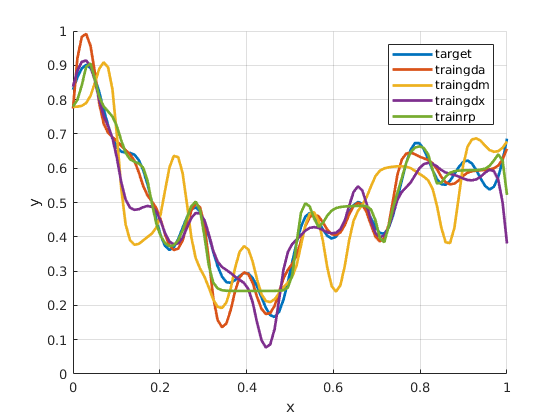
\includegraphics[scale=0.88]{2_6_1}
	\caption{Аппроксимация градиентными алгоритмами}
	\label{fig:2_6_1}
\end{center}
\end{figure}

В таблице \ref{tab:2_6_2} и на рис. \ref{fig:2_6_2} приведены сводные результаты для метода сопряженных градиентов.
\begin{table}[H]
\begin{center}
	\def\tabcolsep{10pt}
	\caption{Метод сопряженных градиентов}
	\label{tab:2_6_2}
	\begin{tabular}{|c|c|c|c|c|}
		\hline
		Функция & Параметры & Нейроны & Ошибка & Число эпох \\
		\hline
		\hline
		\code{traincgf} & \makecell{
			\code{searchFcn = 'srchcha'} \\
			\code{scale_tol = 20} \\
			\code{alpha = 0.001} \\
			\code{beta = 0.1} \\
			\code{delta = 0.01} \\
			\code{gama = 0.1} \\
			\code{low_lim = 0.1} \\
			\code{up_lim = 0.8} \\
			\code{max_step = 100} \\
			\code{min_step = 1.0e-6} \\
			\code{bmax = 26} \\
			\code{batch_frag = 0}} & 25 & 9.3685e-04 & 39 \\
		\hline
		\code{trainscg} & \makecell{
			\code{sigma = 5e-5} \\ 
			\code{lambda = 5e-7}} & 20 & 3.8760e-04 & 45 \\
		\hline
	\end{tabular}
\end{center}
\end{table} 
\vspace{-1cm}
\begin{figure}[H]
\begin{center}
	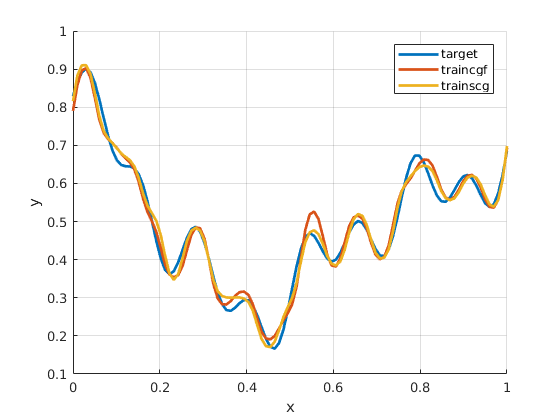
\includegraphics[scale=0.88]{2_6_2}
	\caption{Аппроксимация методом сопряженных градиентов}
	\label{fig:2_6_2}
\end{center}
\end{figure}

В таблице \ref{tab:2_6_3} и на рис. \ref{fig:2_6_3} приведены сводные результаты для квазиньютоновских алгоритмов.
\begin{table}[H]
\begin{center}
	\def\tabcolsep{10pt}
	\caption{Квазиньютоновские алгоритмы}
	\label{tab:2_6_3}
	\begin{tabular}{|c|c|c|c|c|}
		\hline
		Функция & Параметры & Нейроны & Ошибка & Число эпох \\
		\hline
		\hline
		\code{trainbfg} & \makecell{
			\code{searchFcn = 'srchbac'} \\
			\code{scale_tol = 20} \\
			\code{alpha = 0.001} \\
			\code{beta = 0.1} \\
			\code{delta = 0.01} \\
			\code{gama = 0.1} \\
			\code{low_lim = 0.1} \\
			\code{up_lim = 0.8} \\
			\code{max_step = 100} \\
			\code{min_step = 1.0e-6} \\
			\code{bmax = 26} \\
			\code{batch_frag = 0}} & 15 & 4.4726e-04 & 89 \\
		\hline
		\code{trainlm} & \makecell{
			\code{mu = 0.001} \\ 
			\code{mu_dec = 0.1} \\
			\code{mu_inc = 10} \\
			\code{mu_max = 1e10}} & 20 & 6.1573e-05 & 11 \\
		\hline
		\code{trainoss} & \makecell{
			\code{searchFcn = 'srchbac'} \\
			\code{scale_tol = 20} \\
			\code{alpha = 0.001} \\
			\code{beta = 0.1} \\
			\code{delta = 0.01} \\
			\code{gama = 0.1} \\
			\code{low_lim = 0.1} \\
			\code{up_lim = 0.8} \\
			\code{max_step = 100} \\
			\code{min_step = 1.0e-6} \\
			\code{bmax = 26} \\
			\code{batch_frag = 0}} & 15 & 6.8439e-04 & 118 \\
		\hline
	\end{tabular}
\end{center}
\end{table}

Из результатов видно, что наименьшей ошибки на тестовой выборке за относительно небольшое количество шагов достигли квазиньютоновские методы и метод сопряженных градиентов.

\begin{figure}[H]
\begin{center}
	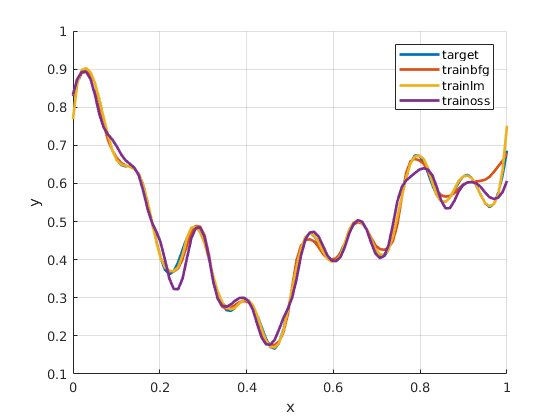
\includegraphics[scale=0.88]{2_6_3}
	\caption{Аппроксимация квазиньютоновскими алгоритмами}
	\label{fig:2_6_3}
\end{center}
\end{figure}
\vspace{-1cm}

\subsection{НС с двумя скрытыми слоями}

%Создайте НС с двумя скрытыми слоями. На 1-2 функциях обучения подберите количество нейронов в 2 скрытых слоях так, чтобы минимизировать ошибку аппроксимации. Сравните количество скрытых нейронов в НС с 1 и 2 скрытыми слоями. Постройте полученный график аппроксимации и приведите значение ошибки.

Создадим НС с двумя скрытыми слоями. Подберем количество нейронов в скрытых слоях для аппроксимации нелинейной функции.
\vspace{-1cm}
\begin{figure}[H]
\begin{center}
	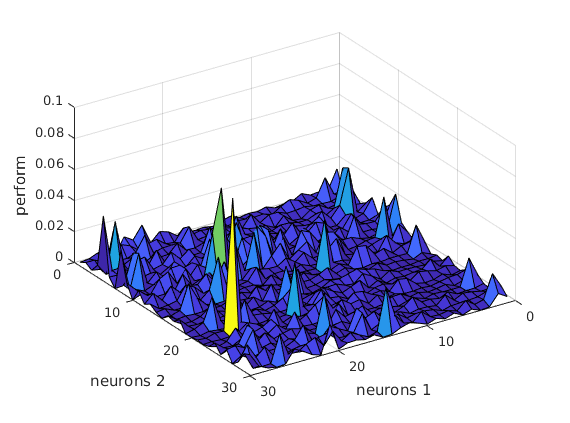
\includegraphics[scale=0.88]{2_7_1}
	\caption{Зависимость ошибки от числа нейронов скрытом слое}
	\label{fig:2_7_1}
\end{center}
\end{figure}

Из графика видно, что нейронная сеть лучше всего минимизирует ошибку при среднем количестве нейронов в обоих слоях, т.е. примерно при $10$ нейронах. В данном случае минимальная ошибка на тестовой выборе была получена при $9$ нейронах в первом скрытом слое и $9$ во втором: ошибка оказалась равна $3.5599\cdot 10^{-5}$, что лучше, чем ошибка, полученная после обучения однослойной нейронной сети ($\approx 10^{-4}$). На рис. \ref{fig:2_7_2} изображены примеры удачной и неудачной аппроксимации.

\begin{figure}[H]
\begin{center}
	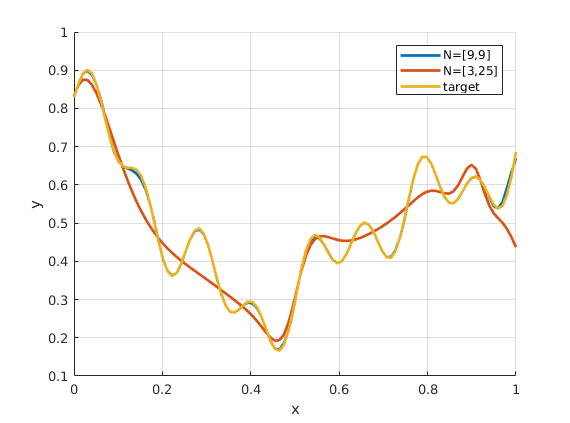
\includegraphics[scale=0.9]{2_7_2}
	\caption{Аппроксимации при различном количестве нейронов}
	\label{fig:2_7_2}
\end{center}
\end{figure}

\newpage

\section{Разбиение плоскости на $2$ класса}

\subsection{Формирование обучающей и тестовой выборки}

Сформируем обучающую и тестовую выборки на основе ранее созданных функций. На рис. \ref{fig:3_1} изображены сформированные выборки.
\begin{figure}[H]
\begin{center}
	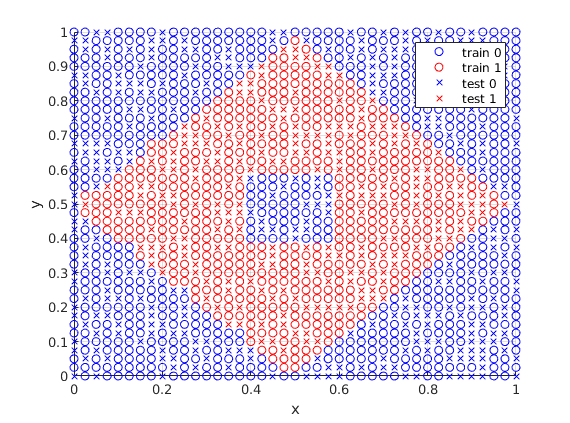
\includegraphics[scale=1]{3_1}
	\caption{Обучающая и тестовая выборки}
	\label{fig:3_1}
\end{center}
\end{figure}

\subsection{Функция обучения и число скрытых нейронов}
\label{sec:inner_neurons}

Для разных функций обучения (\code{trainlm}, \code{trainbfg}, \code{traingdx}, \code{traincgf}) определим оптимальное число нейронов в скрытом слое (слоях), настройте параметры функций обучения, обучите НС, вычислим ошибку классификации.

На рис. \ref{fig:3_2_1} изображена зависимость ошибки от числа нейронов в скрытом слое для различных функций обучения.
\begin{figure}[H]
\begin{center}
	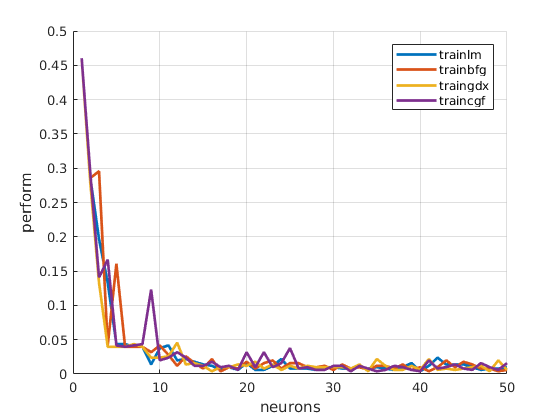
\includegraphics[scale=0.88]{3_2_1}
	\caption{Зависимость ошибки от числа нейронов в скрытом слое}
	\label{fig:3_2_1}
\end{center}
\end{figure}
Из графика видно, что оптимальным для каждой функции обучения является около $20 \div 30$ нейронов. Будем изменять параметры функций обучения при этом количестве нейронов во внутреннем слое. На рис. \ref{fig:3_2} приведены примеры получаемых разбиений. 
\begin{figure}[H]
\begin{center}
	\begin{subfigure}[b]{0.49\textwidth}
		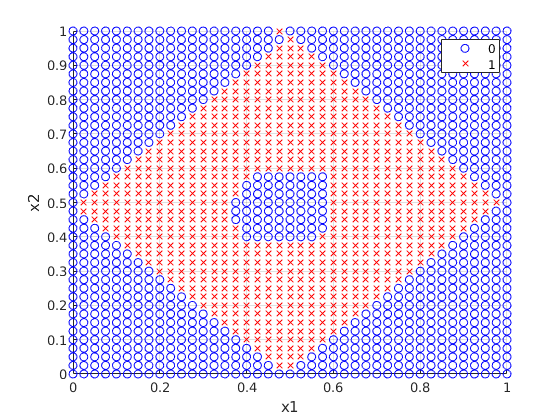
\includegraphics[width=1\textwidth, height=6cm]{3_2_2}
		\caption{Хорошее}
	\end{subfigure}
	\begin{subfigure}[b]{0.49\textwidth}
		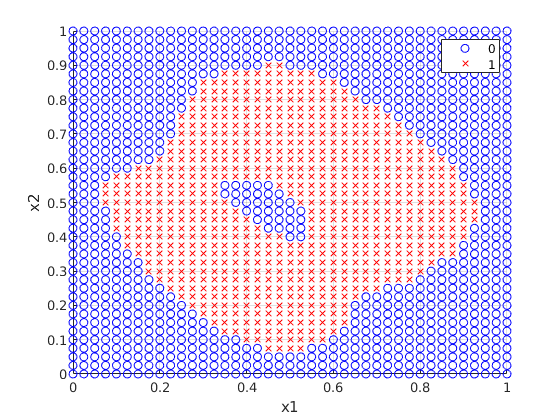
\includegraphics[width=1\textwidth, height=6cm]{3_2_3}
		\caption{Плохое}
	\end{subfigure}
	\caption{Примеры разбиений}
	\label{fig:3_2}
\end{center}
\end{figure}
В таблице \ref{tab:3_2_1} приведены сводные результаты для разных алгоритмов обучения.
\begin{table}[H]
\begin{center}
	\def\tabcolsep{10pt}
	\caption{Различные функции обучения}
	\label{tab:3_2_1}
	\begin{tabular}{|c|c|c|c|c|}
		\hline
		Функция & Параметры & Нейроны & Ошибка & Число эпох \\
		\hline
		\hline
		\code{trainlm} & \makecell{
			\code{mu = 0.01} \\ 
			\code{mu_dec = 0.01} \\ 
			\code{mu_inc = 100} \\
			\code{mu_max = 1e10}} & 35 & 0.079 & 66 \\
		\hline
		\code{trainbfg} & \makecell{
			\code{searchFcn = 'srchbac'} \\
			\code{scale_tol = 20} \\
			\code{alpha = 0.01} \\
			\code{beta = 0.1} \\
			\code{delta = 0.01} \\
			\code{gama = 0.1} \\
			\code{low_lim = 0.2} \\
			\code{up_lim = 0.5} \\
			\code{max_step = 100} \\
			\code{min_step = 1.0e-6} \\
			\code{bmax = 26} \\
			\code{batch_frag = 0}} & 35 & 0.040 & 61 \\
		\hline
		\code{traingdx} & \makecell{
			\code{lr = 0.05} \\
			\code{mc = 0.5} \\
			\code{lr_inc = 1.1} \\
			\code{lr_dec = 0.8} \\
			\code{max_perf_inc  = 1.02}} & 45 & 0.037 & 53 \\
		\hline
		\code{traincgf} & \makecell{
			\code{searchFcn = 'srchbre'} \\
			\code{scale_tol = 50} \\
			\code{alpha = 0.05} \\
			\code{beta = 0.5} \\
			\code{delta = 0.01} \\
			\code{gama = 0.5} \\
			\code{low_lim = 0.2} \\
			\code{up_lim = 0.5} \\
			\code{max_step = 100} \\
			\code{min_step = 1.0e-6} \\
			\code{bmax = 56} \\
			\code{batch_frag = 0}} & 20 & 0.040 & 73 \\
		\hline
	\end{tabular}
\end{center}
\end{table}

Из таблицы видно, что все алгоритмы смогли достичь ошибки $\sim 10^{-2}$, но наилучших результатов удалось добиться с помощью функции \code{traingdx}.

\subsection{Функция производительности}

Изменим выходной слой НС на \code{softmax}, функцию производительности на \code{crossentropy}, функцию обучения \code{trainscg}. Обучим НС, подобрав наилучшее сочетание остальных параметров.

\lstinputlisting[linerange={15-34}]{lab3_3_2.m}

На рис. \ref{fig:3_3} приведены примеры получаемых разбиений. Очевидно, что у нейронной сети не получается с достаточной точностью разбить плоскость на классы. Получаемая ошибка на тестовой выборке $\geq 0.5$.
\begin{figure}[H]
\begin{center}
	\begin{subfigure}[b]{0.49\textwidth}
		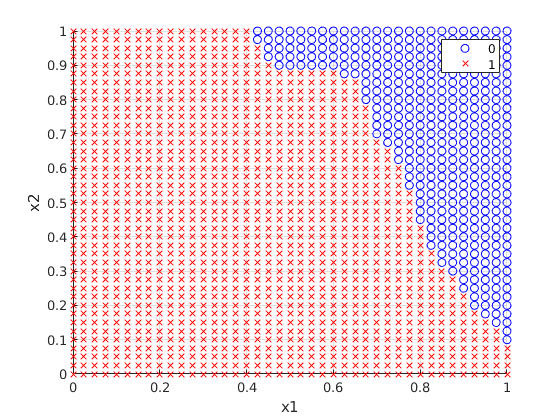
\includegraphics[width=\textwidth, height=6cm]{3_3_1}
		\caption{Плохое}
	\end{subfigure}
	\begin{subfigure}[b]{0.49\textwidth}
		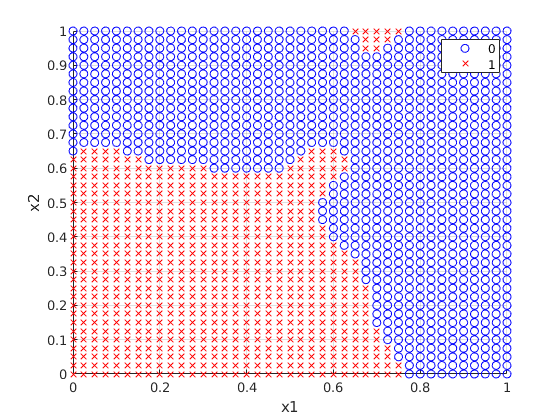
\includegraphics[width=\textwidth, height=6cm]{3_3_2}
		\caption{Плохое}
	\end{subfigure}
	\caption{Примеры разбиений}
	\label{fig:3_3}
\end{center}
\end{figure}

\subsection{Передаточная функция выходного слоя}

Для стандартной функции производительности \code{sse} будем изменять тип передаточной функции выходного слоя на \code{purelin}, \code{tansig} и \code{logsig}. В таблице \ref{fig:3_4} приведены сводные результаты для разных функции производительности.

\begin{table}[H]
\begin{center}
	\def\tabcolsep{15pt}
	\caption{Различные функции производительности}
	\label{tab:3_4}
	\begin{tabular}{|c|c|c|c|}
		\hline
		Функция & Нейроны & Ошибка & Число эпох \\
		\hline
		\hline
		\code{purelin} & 20 & 7 & 348 \\
		\hline
		\code{tansig} & 35 & 13 & 1689 \\
		\hline
		\code{logsig} & 25 & 6 & 1865 \\
		\hline
	\end{tabular}
\end{center}
\end{table}
\vspace{-0.5cm}

На рис. \ref{fig:3_4} приведены примеры разбиений для разных функции производительности.
\vspace{-0.5cm}
\begin{figure}[H]
\begin{center}
	\begin{subfigure}[b]{0.49\textwidth}
		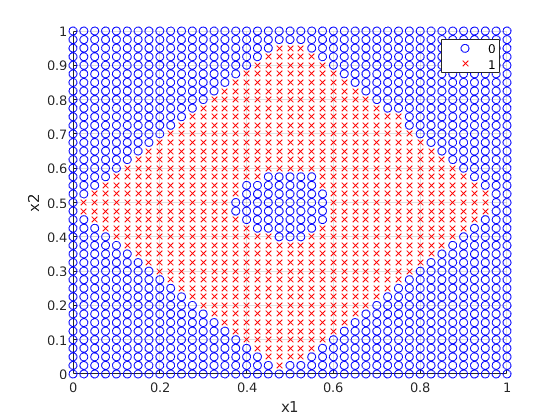
\includegraphics[width=\textwidth, height=6cm]{3_4_purelin}
		\caption{\code{purelin}}
	\end{subfigure}
	\begin{subfigure}[b]{0.49\textwidth}
		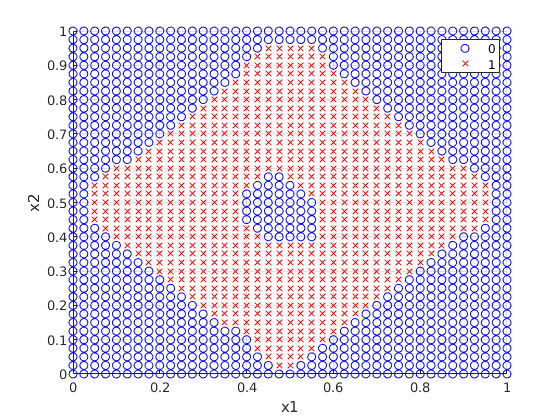
\includegraphics[width=\textwidth, height=6cm]{3_4_tansig}
		\caption{\code{tansig}}
	\end{subfigure}
	\begin{subfigure}[b]{0.49\textwidth}
		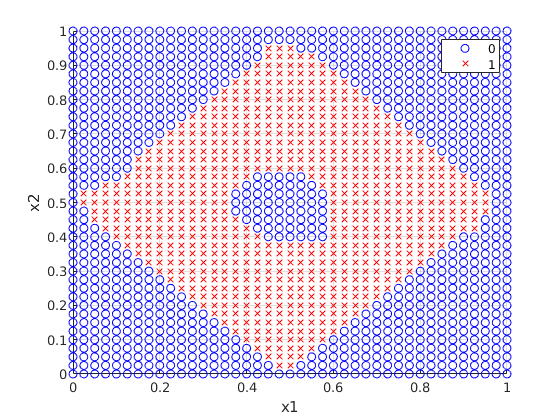
\includegraphics[width=\textwidth, height=6cm]{3_4_logsig}
		\caption{\code{logsig}}
	\end{subfigure}
	\caption{Примеры разбиений для разных функции производительности}
	\label{fig:3_4}
\end{center}
\end{figure}

\subsection{Каскадная НСПР}

Рассмотрим одну из полученных выше конфигураций НС и параметров. Изменим тип нейронной сети на каскадный. На рис. \ref{fig:3_5_1} приведена архитектура каскадной сети.
\begin{figure}[H]
\begin{center}
	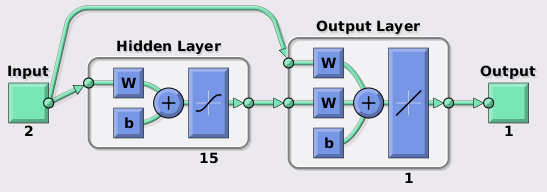
\includegraphics[scale=0.6]{3_5_1}
	\caption{Архитектура каскадной сети}
	\label{fig:3_5_1}
\end{center}
\end{figure}

На рис. \ref{fig:3_5_2} приведен пример разбиения плоскости на классы каскадной нейронной сетью после обучения. При этом ошибка \code{mse} на тестовой выборке оказалась равна $0.0198$, а обучение заняло $1927$ эпох.
\begin{figure}[H]
\begin{center}
	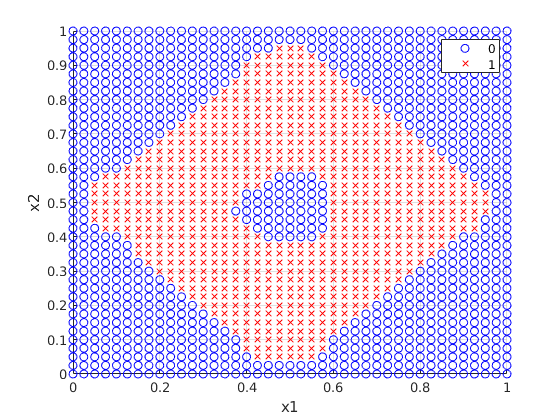
\includegraphics[scale=0.8]{3_5_2}
	\caption{Разбиение на классы}
	\label{fig:3_5_2}
\end{center}
\end{figure}

\section{Разбиение плоскости на $N$ классов}

\subsection{Формирование обучающей и тестовой выборки}

Сформируем обучающую и тестовую выборки на основе ранее созданных функций. На рис. \ref{fig:4_1} изображены сформированные выборки: обучающая выборка обозначена ноликами, а тестовая -- крестиками.
\begin{figure}[H]
\begin{center}
	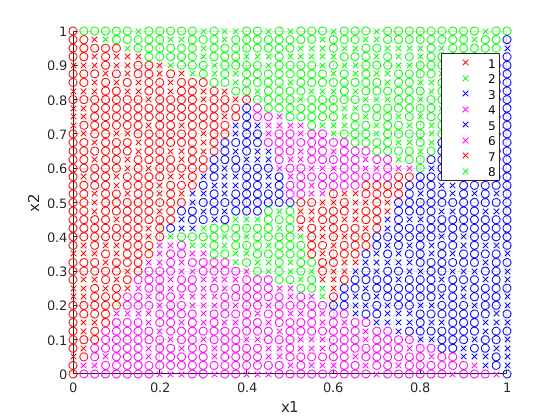
\includegraphics[scale=1]{4_1}
	\caption{Обучающая и тестовая выборки}
	\label{fig:4_1}
\end{center}
\end{figure}

\subsection{Функция обучения и число скрытых нейронов}

Для разных функций обучения (\code{trainlm}, \code{trainbfg}, \code{traingdx}, \code{traincgf}) определим оптимальное число нейронов в скрытом слое (слоях), настройте параметры функций обучения, обучите НС, вычислим ошибку классификации.

На рис. \ref{fig:3_2_1} изображена зависимость ошибки от числа нейронов в скрытом слое для различных функций обучения.
\begin{figure}[H]
\begin{center}
	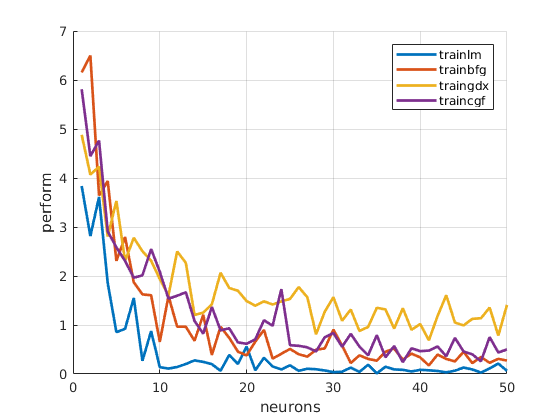
\includegraphics[scale=0.88]{4_2_1}
	\caption{Зависимость ошибки от числа нейронов в скрытом слое}
	\label{fig:4_2_1}
\end{center}
\end{figure}
Таким образом, оптимальное количетсво нейронов оказалось следующим: \code{trainlm} -- 34 нейрона, \code{traunbfg} -- 23 нейрона, \code{traingdx} -- 36 нейронов, \code{traincgf} -- 46 нейрнов. Оптимальные параметры функций обучения, в данном случае, оказались теми же, что и в разделе \ref{sec:inner_neurons}, при этом ошибки \code{mse} оказались равны: \code{trainlm} -- 0.0298, \code{traunbfg} -- 0.0794, \code{traingdx} -- 0.0951, \code{traincgf} -- 0.0476. На рис. \ref{fig:4_2} изображены примеры получаемых разбиений.
\begin{figure}[H]
\begin{center}
	\begin{subfigure}[b]{0.49\textwidth}
		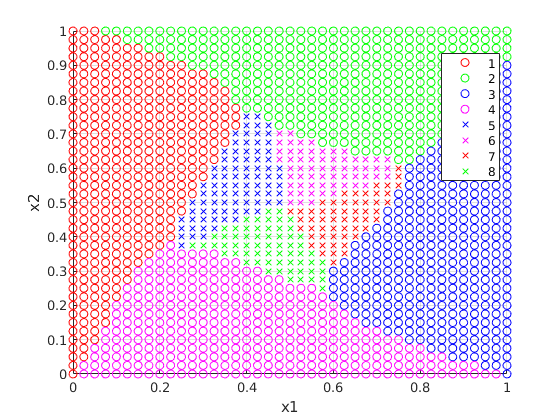
\includegraphics[width=1\textwidth]{4_2_3}
		\caption{Хорошее}
	\end{subfigure}
	\begin{subfigure}[b]{0.49\textwidth}
		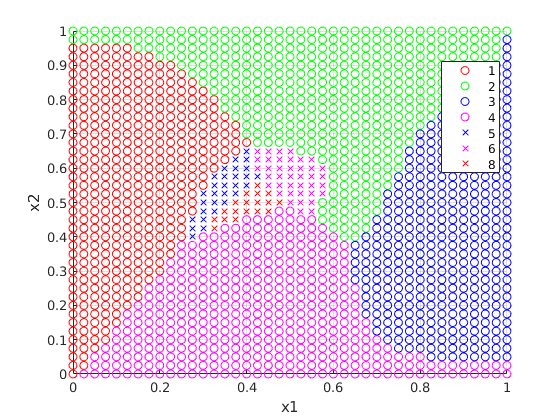
\includegraphics[width=1\textwidth]{4_2_2}
		\caption{Плохое}
	\end{subfigure}
	\caption{Примеры разбиений}
	\label{fig:4_2}
\end{center}
\end{figure}

\subsection{Функция производительности}

Изменим выходной слой НС на \code{softmax}, функцию производительности на \code{crossentropy}, функцию обучения \code{trainscg}. Обучим НС, подобрав наилучшее сочетание остальных параметров.

\lstinputlisting[linerange={16-32}]{lab3_4_2.m}

На рис. \ref{fig:4_3} приведены примеры получаемых разбиений. Видно, что исходные прямые, разбивающие плоскость на классы, изменили свои углы наклона, а также уменьшились классы, расположенные по центру. Ошибка на тестовой выборке оказалась равна $1.9984 \cdot 10^{-16}$. 
\vspace{-1cm}
\begin{figure}[H]
\begin{center}
	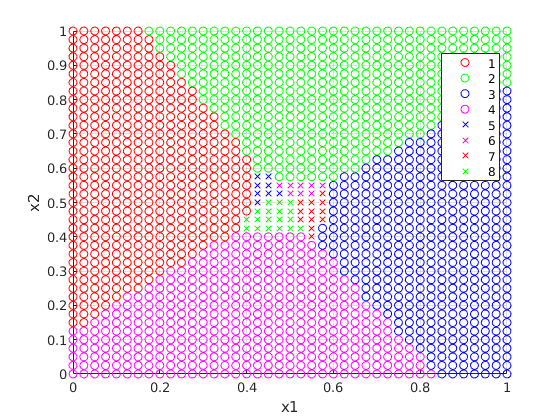
\includegraphics[width=0.75\textwidth]{4_3}
	\caption{Пример разбиения}
	\label{fig:4_3}
\end{center}
\end{figure}

\subsection{Передаточная функция выходного слоя}

Для стандартной функции производительности \code{sse} будем изменять тип передаточной функции выходного слоя на \code{purelin}, \code{tansig} и \code{logsig}. В таблице \ref{fig:3_4} приведены сводные результаты для разных функции производительности.

\lstinputlisting[linerange={15-32}]{lab3_3_4.m}

\begin{table}[H]
\begin{center}
	\def\tabcolsep{15pt}
	\caption{Различные функции производительности}
	\label{tab:3_4}
	\begin{tabular}{|c|c|c|c|}
		\hline
		Функция & Нейроны & Ошибка & Число эпох \\
		\hline
		\hline
		\code{purelin} & 50 & 192 & 443 \\
		\hline
		\code{tansig} & 50 & 209 & 889 \\
		\hline
		\code{softmax} & 35 & 88 & 221 \\
		\hline
		\code{logsig} & 20 & 529 & 483 \\
		\hline
	\end{tabular}
\end{center}
\end{table}

На рис. \ref{fig:3_4} приведены примеры разбиений для разных функции производительности.
\vspace{-0.5cm}
\begin{figure}[H]
\begin{center}
	\begin{subfigure}[b]{0.49\textwidth}
		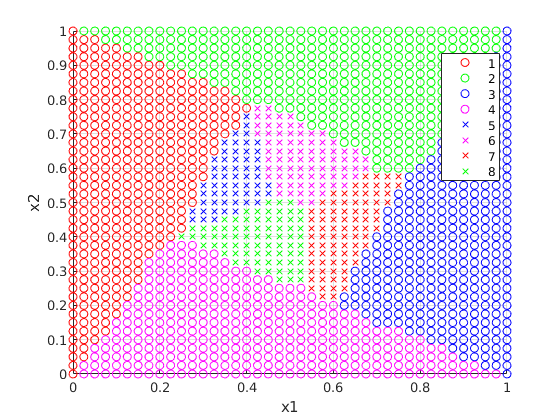
\includegraphics[width=\textwidth]{4_4_purelin}
		\caption{\code{purelin}}
	\end{subfigure}
	\begin{subfigure}[b]{0.49\textwidth}
		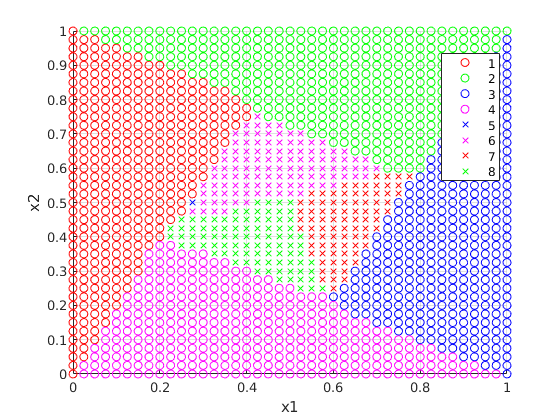
\includegraphics[width=\textwidth]{4_4_tansig}
		\caption{\code{tansig}}
	\end{subfigure}
	\begin{subfigure}[b]{0.49\textwidth}
		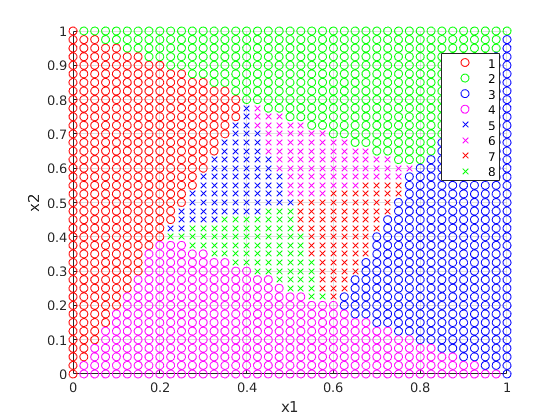
\includegraphics[width=\textwidth]{4_4_softmax}
		\caption{\code{softmax}}
	\end{subfigure}
	\begin{subfigure}[b]{0.49\textwidth}
		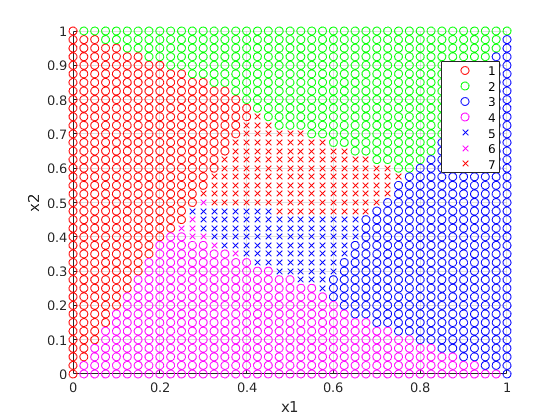
\includegraphics[width=\textwidth]{4_4_logsig}
		\caption{\code{logsig}}
	\end{subfigure}
	\caption{Примеры разбиений}
	\label{fig:4_4}
\end{center}
\end{figure}

\newpage

\subsection{Каскадная НСПР}

Рассмотрим одну из полученных выше конфигураций НС и параметров. Изменим тип нейронной сети на каскадный. На рис. \ref{fig:4_5_1} приведена архитектура каскадной сети.

\begin{figure}[H]
\begin{center}
	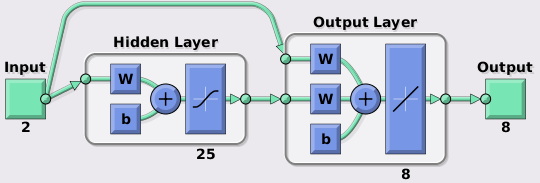
\includegraphics[scale=0.6]{4_5_1}
	\caption{Архитектура каскадной сети}
	\label{fig:4_5_1}
\end{center}
\end{figure}

\vspace{-0.5cm}
Оптимальным оказалось использование 25 нейронов в скрытом слое. На рис. \ref{fig:4_5_2} приведен пример разбиения плоскости на классы каскадной нейронной сетью после обучения. При этом ошибка \code{sse} на тестовой выборке оказалась равна $141$, что несколько лучше, чем результаты, полученные в предыдущем разделе. Обучение при этом заняло $710$ эпох.
\vspace{-0.5cm}
\begin{figure}[H]
\begin{center}
	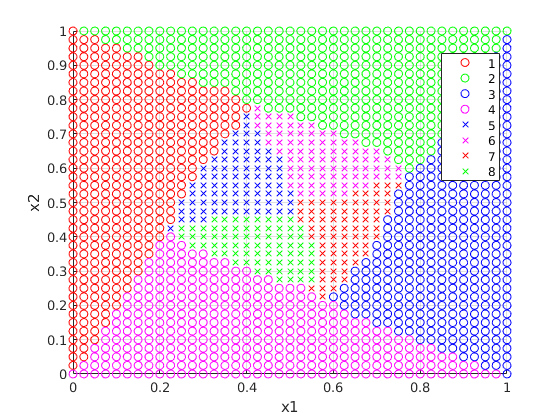
\includegraphics[scale=0.8]{4_5_2}
	\caption{Разбиение на классы}
	\label{fig:4_5_2}
\end{center}
\end{figure}
\vspace{-1cm}

\newpage

\section{Классификация многомерных образов}

%1. В качестве исходных данных используйте задания с номером 8. Размерность входного сигнала совпадает с размерностью изображения. Размерность выходного сигнала – количество классов. Сформируйте обучающую и тестовую выборки достаточного объема. Продумайте 2-3 постановки задачи в зависимости от типа зашумления и искажения (равномерный шум, изменение масштаба, сдвиг, поворот).
%2. Выполните исследования по аналогии с заданием 3. Приведите найденные наилучшие конфигурации нейронных сетей, параметров обучения, а также результаты обучения – матрицы неточностей, ошибки 1,2 рода.

\subsection{Формирование обучающей и тестовой выборки}

Сформируем обучающую и тестовую выборки на основе ранее созданных функций. На рис. \ref{fig:5_1_1} изображены примеры обучающей выборки.
\begin{figure}[H]
\begin{center}
	
\includegraphics[scale=1]{5_1_1}
	\caption{Исходные образы \code{P}}
	\label{fig:5_1_1}
\end{center}
\end{figure}

Сформируем зашумленные образы, повернутые на случайный угол и сдвинутые относительно исходных. На рис. \ref{fig:5_1_2} изображены примеры таких образов.
\begin{figure}[H]
\begin{center}
	\begin{subfigure}[b]{\textwidth}
		
\includegraphics[scale=1]{5_1_2}
		\caption{Зашумленная выборка \code{P_noisy}}
	\end{subfigure}
	\begin{subfigure}[b]{\textwidth}
		
\includegraphics[scale=1]{5_1_3}
		\caption{Повернутая выборка \code{P_rotate}}
	\end{subfigure}
	\begin{subfigure}[b]{\textwidth}
		
\includegraphics[scale=1]{5_1_4}
		\caption{Сдвинутая выборка \code{P_shift}}
	\end{subfigure}
	\caption{Примеры разбиений}
	\label{fig:5_1_2}
\end{center}
\end{figure}

\subsection{Функция обучения и число скрытых нейронов}

Для различных функций обучения (\code{trainlm}, \code{trainbfg}, \code{traingdx}, \code{traincgf}) было определено оптимальное количество нейронов в скрытом слое: \code{trainlm} -- 50 нейронов, \code{trainbfg}, \code{traingdx} и \code{traincgf} -- 100 нейронов. Исходная выборка была поделена в отношении $0.5 : 0.5$ на обучающую и тестовую. Для вычисления ошибки была использована тестовая выборка. На рис. \ref{fig:5_2_1} приведены матрицы неточностей, полученные после обучения этими методами.

\begin{figure}[H]
\begin{center}
	\begin{subfigure}[b]{0.49\textwidth}
		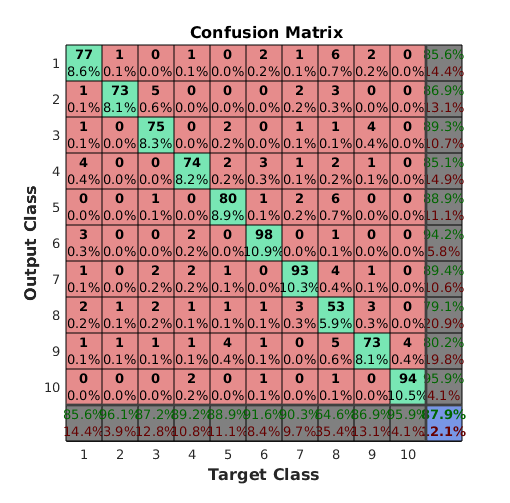
\includegraphics[width=1\textwidth]{5_2_1}
		\caption{\code{trainlm}, err = 0.12}
	\end{subfigure}
	\begin{subfigure}[b]{0.49\textwidth}
		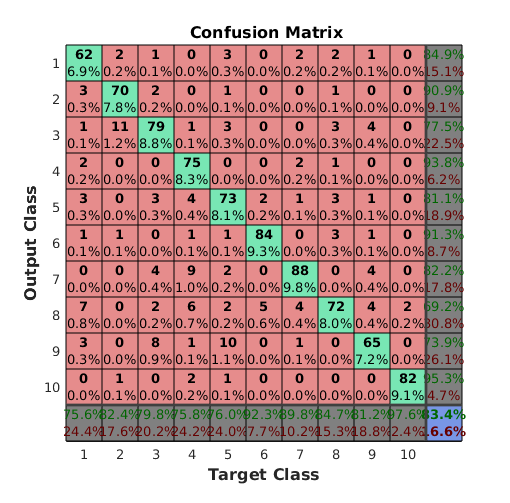
\includegraphics[width=1\textwidth]{5_2_2}
		\caption{\code{trainbfg}, err = 0.16}
	\end{subfigure}
	\begin{subfigure}[b]{0.49\textwidth}
		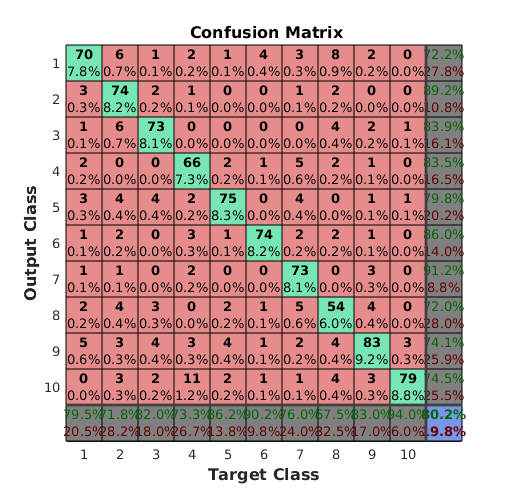
\includegraphics[width=1\textwidth]{5_2_3}
		\caption{\code{traingdx}, err = 0.19}
	\end{subfigure}
	\begin{subfigure}[b]{0.49\textwidth}
		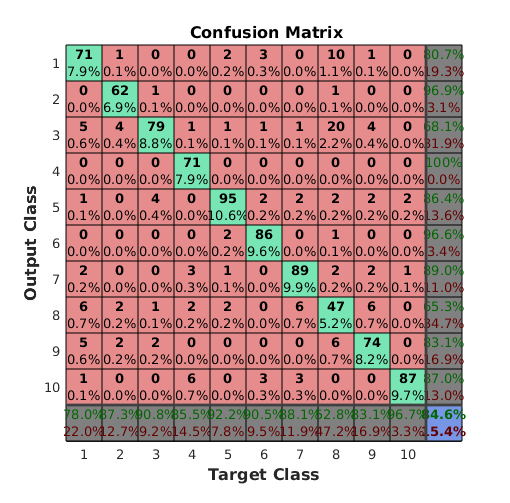
\includegraphics[width=1\textwidth]{5_2_4}
		\caption{\code{traincgf}, err = 0.15}
	\end{subfigure}
	\caption{Матрицы неточностей}
	\label{fig:5_2_1}
\end{center}
\end{figure}

\subsection{Функция производительности}

Изменим выходной слой НС на \code{softmax}, функцию производительности на \code{crossentropy}, функцию обучения \code{trainscg}. Подберем оптимальное число нейронов в скрытом слое. На рис. \ref{fig:5_3_1} изображена зависимость ошибки от числа нейронов в скрытом слое.
\begin{figure}[H]
\begin{center}
	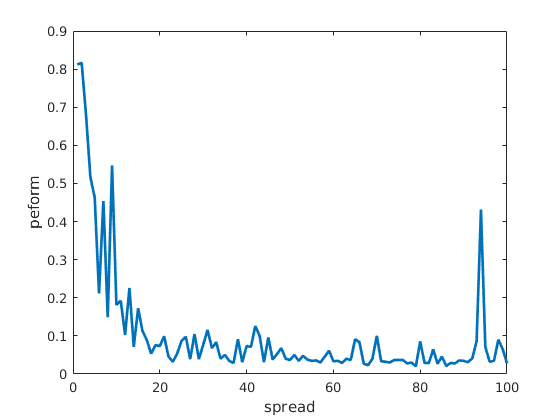
\includegraphics[scale=0.88]{5_3_1}
	\caption{Зависимость ошибки от числа нейронов в скрытом слое}
	\label{fig:5_3_1}
\end{center}
\end{figure}

На рис. \ref{fig:5_3_2} изображена матрица неточностей при оптимальном числе нейронов, равном 50.
\begin{figure}[H]
\begin{center}
	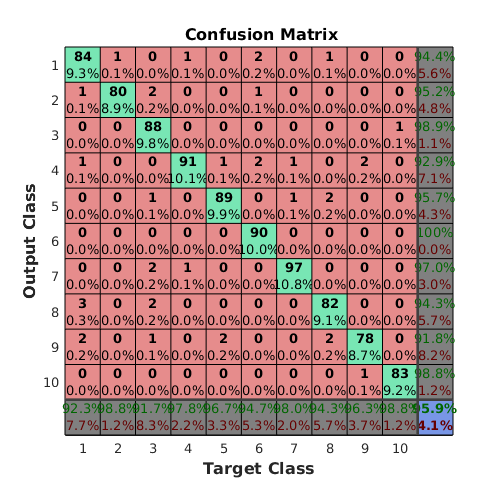
\includegraphics[scale=0.7]{5_3_2}
	\caption{Матрица неточностей, err = 0.041}
	\label{fig:5_3_2}
\end{center}
\end{figure}

\subsection{Передаточная функция выходного слоя}

Для стандартной функции производительности \code{sse} будем изменять тип передаточной функции выходного слоя на \code{purelin}, \code{tansig} и \code{logsig}. В таблице \ref{fig:3_4} приведены сводные результаты для разных функции производительности.

\begin{table}[H]
\begin{center}
	\def\tabcolsep{15pt}
	\caption{Различные функции производительности}
	\label{tab:3_4}
	\begin{tabular}{|c|c|c|c|}
		\hline
		Функция & Нейроны & Ошибка & Число эпох \\
		\hline
		\hline
		\code{purelin} & 100 & 1748 & 329 \\
		\hline
		\code{tansig} & 100 & 1194 & 230 \\
		\hline
		\code{softmax} & 50 & 1684 & 221 \\
		\hline
		\code{logsig} & 100 & 6507 & 176 \\
		\hline
	\end{tabular}
\end{center}
\end{table}
\vspace{-0.5cm}

На рис. \ref{fig:3_4} приведены матрицы неточностей для разных функции производительности.
\vspace{-0.5cm}
\begin{figure}[H]
\begin{center}
	\begin{subfigure}[b]{0.49\textwidth}
		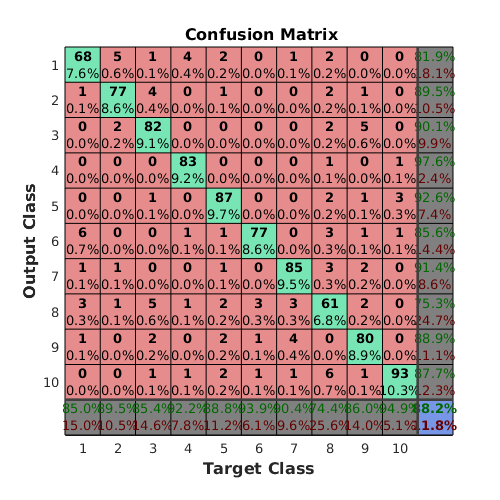
\includegraphics[width=\textwidth]{5_4_1}
		\caption{\code{purelin}}
	\end{subfigure}
	\begin{subfigure}[b]{0.49\textwidth}
		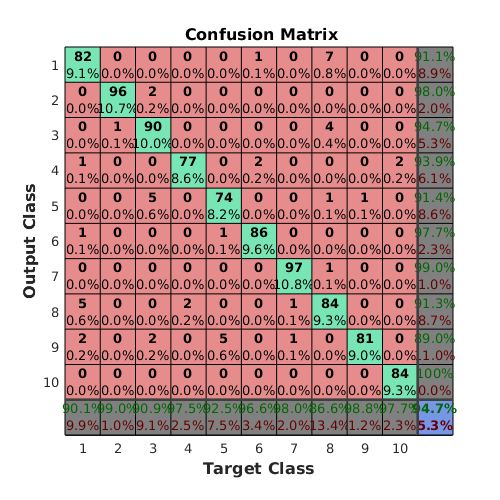
\includegraphics[width=\textwidth]{5_4_2}
		\caption{\code{tansig}}
	\end{subfigure}
	\caption{Матрицы неточностей}
\end{center}
\end{figure}
\begin{figure}[H]
\begin{center}
	\begin{subfigure}[b]{0.49\textwidth}
		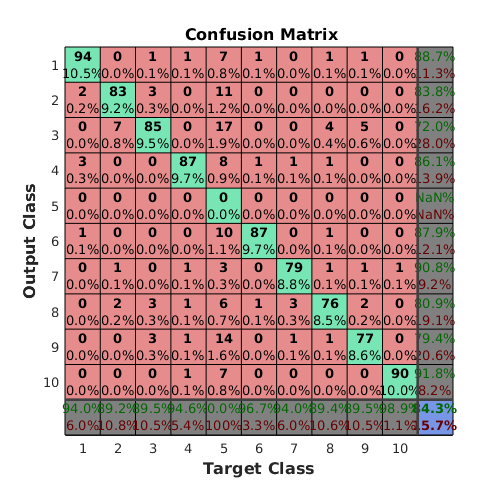
\includegraphics[width=\textwidth]{5_4_3}
		\caption{\code{softmax}}
	\end{subfigure}
	\begin{subfigure}[b]{0.49\textwidth}
		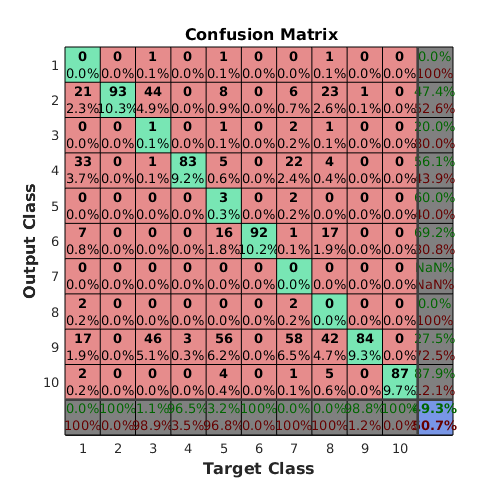
\includegraphics[width=\textwidth]{5_4_4}
		\caption{\code{logsig}}
	\end{subfigure}
	\caption{Матрицы неточностей}
	\label{fig:4_4}
\end{center}
\end{figure}

\subsection{Каскадная НСПР}

Рассмотрим одну из полученных выше конфигураций НС и параметров. Изменим тип нейронной сети на каскадный. На рис. \ref{fig:4_5_1} приведена архитектура каскадной сети.

\begin{figure}[H]
\begin{center}
	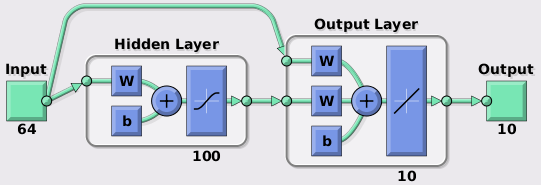
\includegraphics[scale=0.6]{5_5_1}
	\caption{Архитектура каскадной сети}
	\label{fig:4_5_1}
\end{center}
\end{figure}

\vspace{-0.5cm}
На рис. \ref{fig:4_5_2} приведен пример разбиения плоскости на классы каскадной нейронной сетью после обучения. При этом ошибка \code{sse} на тестовой выборке оказалась равна $141$, что несколько лучше, чем результаты, полученные в предыдущем разделе. Обучение при этом заняло $710$ эпох.
\vspace{-0.5cm}
\begin{figure}[H]
\begin{center}
	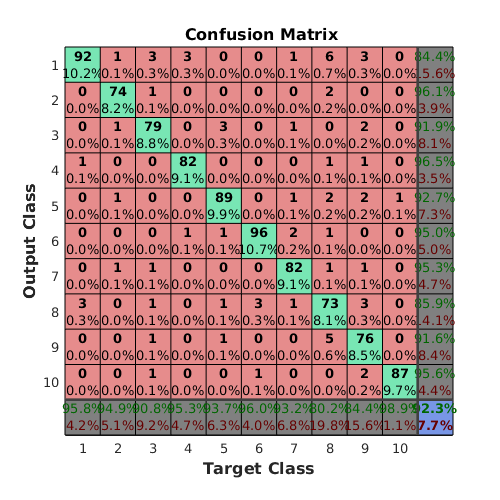
\includegraphics[scale=0.8]{5_5_2}
	\caption{Матрица неточностей, sse = 1252, mse = 0.07}
	\label{fig:4_5_2}
\end{center}
\end{figure}
\vspace{-1cm}

\subsection{Зашумленные входные образы}

С использованием алгоритмы \code{trainlm} (самый низкий процент ошибок в пункте 1) обучим нейронную сеть на исходных образах и проверим качество классификации зашумленных образов, повернутых образов на случайный угол и образов, сдвинутых относительно исходных. На рис. \ref{fig:5_6_1} приведены матрицы неточностей для искаженных выходных образов.
\vspace{-0.3cm}
\begin{figure}[H]
\begin{center}
	\begin{subfigure}[b]{0.47\textwidth}
		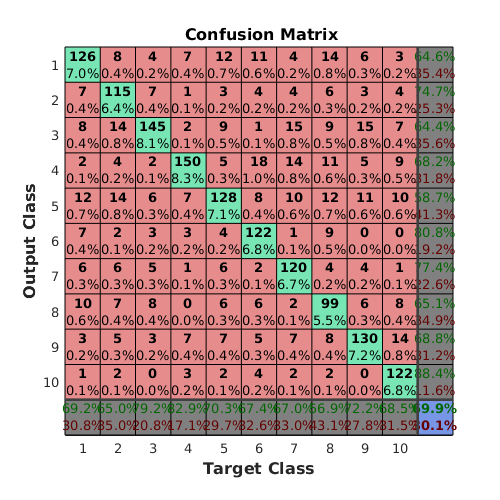
\includegraphics[width=\textwidth]{5_6_1}
		\caption{Шум, err = 0.3}
	\end{subfigure}
	\begin{subfigure}[b]{0.47\textwidth}
		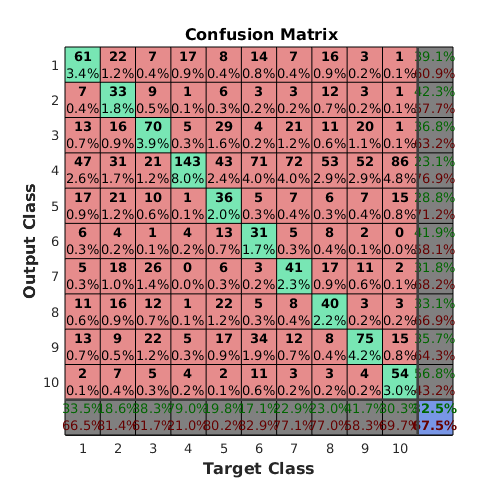
\includegraphics[width=\textwidth]{5_6_2}
		\caption{Поворот, err = 0.67}
	\end{subfigure}
\end{center}
\end{figure}
\begin{figure}[H]
\begin{center}
	\begin{subfigure}[b]{0.49\textwidth}
		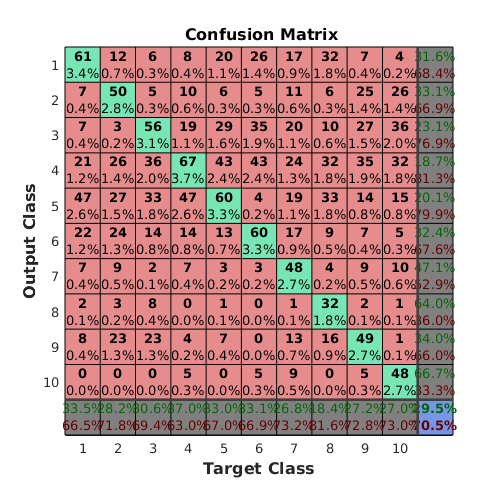
\includegraphics[width=\textwidth]{5_6_3}
		\caption*{(c) Сдвиг, err = 0.7}
	\end{subfigure}
	\caption{Матрицы неточностей}
	\label{fig:5_6_1}
\end{center}
\end{figure}

Как видно из результатов классификации, нейронная сеть оказалась очень чувствительна к поворотам и сдвигам изображения, в то время как даже зашумления не вызывали настолько сильного ухудшения классификации. 

\section{Выводы}

В процессе выполнения данной работы были приобретены навыки построения и инициализации нейронных сетей прямого распространения. Рассмотрены различные функции обработки входных и выходных сигналов. Изучены различные функции расчета производительности НС и деления выборки. Получен опыт практического применения сетей прямого распространения и их обучения с использованием алгоритма обратного распространения ошибки.

\end{document}